\section{Introduction}\label{sec:intros}

Vulnerabilities due to memory corruption are still a major issue for C programs~\cite{cvetrend, microsoftmemsafe, Zeng:2013:SRF:2534766.2534798}  despite many efforts that tried to prevent them~\cite{song2019sanitizing}.
These vulnerabilities are not uniformly distributed in real programs~\cite{meng2021bran, du2019leopard},
as some components are likelier to have a certain class of vulnerabilities.
\eg{} spatial safety issues in string processing functions.

Program partitioning enables separating potentially vulnerable functions (untrusted region) from the rest of the program (trusted region).
Several program partitioning mechanisms~\cite{tan2017principles, brumley2004privtrans, bittau2008wedge, lind2017glamdring, liu2017ptrsplit,rlbox-paper,10.1145/3492321.3519582,privtrans,cqual-kernel-ptr,10.1145/3371100} exist.
These techniques usually combine program partitioning with SFI to guarantee robust safety \cite{10.1145/3371100}, such that code in the untrusted region cannot affect code in the trusted region,~\eg{} by executing untrusted partition in a separate process~\cite{liu2017ptrsplit} or executing in a trusted execution environment~\cite{lind2017glamdring}. 

Unfortunately, the robust safety statement is too vague in expressing the exact safety it provides, and it causes the systems based on it --- such as the ones above --- provide stronger guarantees than they should be and cause considerable performance overhead, but also provide ways where users can reduce overhead by essentially violating the robust safety.
For example, RLBox \cite{rlbox-paper} and PKRU-Safe \cite{10.1145/3492321.3519582} have a $100\%$ - $200\%$ overhead, and RLbox permits users to bypass its verification procedures that guarantee robust safety.
The ambiguity and its associated performance drawback decelerates the mechanism's development \cite{sandboxfu}.

In all these program partitioning mechanisms, the program partitioning parts are clear and similar.
They provided a type system or user defined annotations to permit the identification of untrusted data, perform some memory separation techniques (separate heaps or sandbox mechanism) to separate the allocations of trusted and untrusted data, and insert dynamic checks to restrict the communications of these two data.
The differences in these mechanisms appeared in the SFI part for separating completely the trusted and untrusted regions that respectively contain trusted and untrusted data, as well as the user defined verification procedures for the permission of some untrusted data usage in trusted regions, which are also the performance bottlenecks.
To balance safety guarantees and performance overhead, we first need to investigate the guarantees that program partitioning can provide, without the involvement of SFI.

In a program partitioning mechanism, a program is split into two regions: a \umode~\emph{region} representing the untrusted partition, and the \cmode~\emph{region} representing the trusted partition. Typically, there is a special types of pointers, which we named \textbf{tainted} (\tmode) mode pointers, being introduced to be used in communicating the \umode and \cmode regions, i.e.,
untainted pointers cannot be used in \umode region, while there are checks requiring for \tmode mode pointers to be used in \cmode region.
Users annotate pointer types and there is a static procedure, such as type checking, then creates two sets of source files:~\ucregion{} and~\cregion{}, containing tainted and untainted entities, respectively.
In addition, untainted pointers that are used in \cmode region are typically viewed as "good" pointers, named \emph{checked} (\cmode mode) pointers. Users classify \cmode mode pointers and \cmode region in a program because they consider these entities are safe to use, which indicates that the guarantee assumptions in \cmode and \umode regions are different and the safety property should reflect such differences.

We present \systemname, as a formalism for the above type-directed program partitioning mechanism based on \checkedc,
and show that the memory safety the mechanism provides is the \emph{non-crashing} property, i.e.,
\cmode region never experiences crashing due to memory safety issues regardless the execution of \umode region.
We also show that the system provides \emph{clean separation} property as a corollary of the non-crashing property,
i.e., any memory violation in \umode region does not affect the execution of \cmode region.


The system is based on \checkedc because of the third concern above. In privilege separation, it is obvious that trusted code is viewed as the part that does not have problem, while programs are in untrusted code, which is similar to the concept of checked and unchecked code regions in \checkedc and make it a perfect model to formalize type-directed program partitioning.
We make precise about the guarantees that a program partition mechanism can provide and have the following contributions.

\myparagraph{\systemname Type System and Formalism}
We present a type system that integrates tainted types with~\checkedc and provides additional guarentees---the~\emph{non-crashing} and \emph{non-exposure} guarantees,~\ie a well-typed~\systemname program can never crash due to spatial safety violations,
as well as \ucregion code cannot directly observe a checked pointer address.
%no \cregion pointer addresses will be leaked in
%\ucregion code
We extend the \checkedc compiler to support the type system and
formalize it by extending~\checkedc formalism~\cite{li22checkedc} with the non-crashing and non-exposure guarantees.
We formally prove theorems related to the two guarantees and use model-based randomized testing \cite{Pierce:SF4} to certify the simulation relation between the~\systemname semantics and its compiler formalism.
To the best of our knowledge,~\systemname is the first C(-like) language and compiler formalism with the program partitioning mechanism.


We designed and implemented a flexible program partition technique using tainted types.
Our type system guarantees that the tainted pointers cannot affect untainted pointers and partition the given code into~\ucregion (containing only tainted entities) and~\cregion (CITE SECTION).
We provide formal proof of the~\emph{clean separation theorem} that guarantees that code in ~\cregion will be separated from~\ucregion according to the target isolation mechanism (CITE SECTION).
We also integerated~\systemname{} with~\checkedc that provides additional~\emph{non-crashing} and \emph{non-exposure} guarantees (CITE SECTION).

\myparagraph{Sound and Better Compilation} Our second
contribution is a formalization of bounds-check insertion for array
accesses (Section~\ref{sec:compilation}). Our operational semantics
annotates each pointer with metadata that describes its bounds, and
the assignment and dereference rules have premises to confirm the
access is in bounds. An obvious compilation scheme (taken by
Cyclone~\cite{Jim2002,GrossmanMJHWC02}, CCured~\cite{Necula2005}, and
earlier works) would be to translate annotated pointers to multi-word
objects: one word for the pointer, and 1-2 words to describe its lower
and upper bounds. Inserted checks reference these bounds. While
convenient, such ``fat'' pointers are expensive, and break backward
binary compatibility with legacy pointers.

  To show that pointer annotations can be safely
  erased, and thus fat pointers are not needed, we formalize a
  translation of \lang to \elang, which is an 
  untyped version of \lang that drops metadata annotations, and
  lacks bounds/null checks in the semantics rules. Instead,
  the compilation process inserts null/bounds checks explicitly, leveraging
  compile-time type information. While we do not definitively prove
  it, we provide strong evidence that compilation is correct. We use PLT
  Redex~\cite{pltredex} to mechanize (a generalization of) \lang, 
  \elang, and compilation between the two, and we use randomized testing 
to validate that the compiled program \emph{simulates} the
original. In addition to demonstrating the technical point that metadata
annotations in the \lang formalism do not necessitate fat pointers,
compilation also sheds light on the actual Checked C compilation
process. 
% \review{ Beginning of page 2: "we show", then "give confidence". I am left confused as
%   to whether the CoreChkC --> CoreC compilation is shown correct (theorem with
%   proof), or carefully debugged and tested in plt-redex (which is fine too, I
%   just find the choice of terminology confusing)}
% \liyi{typo, should be "validate through randomized testing"}

As far as we are aware, \lang is the first formalism to cleanly
separate bounds-checking compilation from the core semantics; prior
work~\cite{Feng2006,Condit2007} merged the two, conflating
\emph{meaning} with \emph{mechanism}. In carrying out the
formalization, we discovered that our compilation approach for
null-terminated array pointers is more expressive than that proposed
in the Checked C specification~\cite{checkedc}
(Section~\ref{sec:disc}); we would not have discovered this
improvement had we not separated checks from semantics.

With the understanding of the true guarantees from program partitioning, we find a better compilation strategy.
Instead of sanitizing the entire \umode region, as many previous mechanisms did \cite{rlbox-paper},
we can only sanitize the \tmode pointers by providing extra dynamic checks in the compiler.
Compared to a typical $100\%$ - $200\%$ overhead in these works \cite{rlbox-paper} as our faithful RLBox representation \systemnamea,
we show that the new compilation implementation, named \systemnameh, only having an average $5\%$ overhead compared to the original \checkedc compiler.

\myparagraph{Extending \checkedc}
We formalize \systemname in \checkedc \cite{li22checkedc} because it has a formalism and compilation.
More importantly, \checkedc has checked and unchecked regions coinciding with the \cmode and \umode regions in program partitioning,
and it provides spatial safety for \cmode region and guarantees that any memory violation is from \umode region,
which is similar to the concept that \cmode region contains only "good" pointers.
Based on the \checkedc formalism, we provide extra \tmode mode pointers to communicate the \cmode and \umode regions in \checkedc, while keeping the original \cmode and \umode mode pointers to be only used in \cmode and \umode regions, respectively.
By upgrading the \checkedc formalism to \systemname, we not only build the foundation for program partitioning, but also extends \checkedc
to support safeties for third party libraries. Previously, users are required to rewrite C code to \checkedc completely to guarantee memory safeties. With \systemname, users can view C library functions as \umode region, and utilize \systemname to validate the \tmode mode pointers returning from these \umode region, without painfully rewriting the C library functions to \checkedc.


\begin{figure}
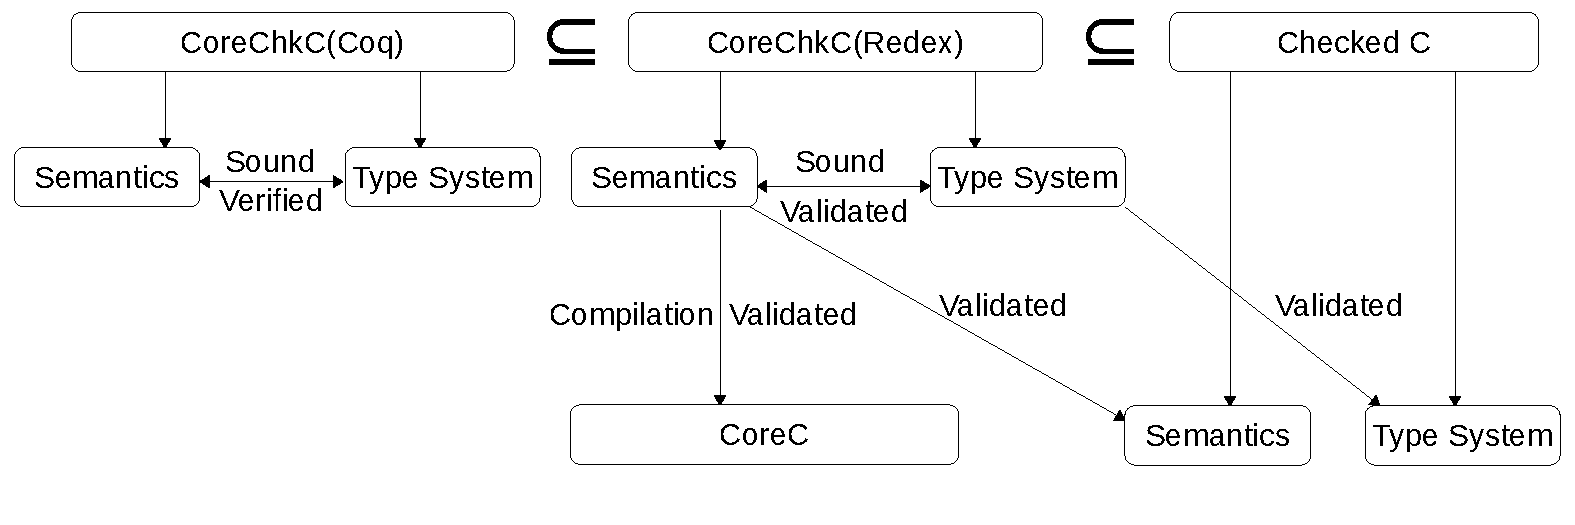
\includegraphics[width=0.5\textwidth]{relationship.pdf}
\caption{
    \lang models' relationship to \checkedc
}
  \label{fig:model-relation}
\end{figure}

\myparagraph{Summary Visualization} The
  relationship among our contributions is visualized in
  Fig.~\ref{fig:model-relation}. With the Coq model of \lang we prove
  soundness (and with it, \emph{blame}) of the \checkedc type system
  and semantics. With the Redex model, we use randomized testing to
  validate both type soundness and compilation correctness, where the
  latter shows how compilation need not output fat pointers despite
  the use of pointer annotations in the \lang model. The Redex \lang
  model is also the basis of randomized testing of the correctness of
  the \checkedc compiler implementation, both its type checker and the
  semantics of its emitted code, at least for the subset of the
  language in the Redex model. The Redex model's syntax
  is slightly richer than the Coq version: conditional guards and
  function arguments may be arbitrary expressions, where the Coq
  version limits them to constants and variables, making handling of
  dependent types a bit simpler. We find a useful synergy between the
  Coq and Redex models for carrying out a language development. The
  richer, executable Redex model is useful for quickly modeling and
  testing new features, both formally and against a real
  implementation. Once solidified, new features can be added to the
  Coq model (perhaps somewhat simplified) for final proofs of
  correctness.

We begin with a review of \checkedc (Section~\ref{sec:overview}),
present our main contributions
(Sections~\ref{sec:formal}--\ref{sec:evaluation}), and conclude with a
discussion of 
related and future work (Sections~\ref{sec:related},
\ref{sec:conclude}). All code and proof artifacts (both for Coq and
Redex) can be found at \url{https://github.com/plum-umd/checkedc}. 










